\documentclass{ctexart}

\usepackage{setspace}
\usepackage{booktabs}
\usepackage{amsmath,amsfonts,amsthm}
\usepackage{tcolorbox}
\usepackage{tikz}
\usepackage{enumitem}
\usepackage{float}
\usepackage{graphicx}

\setlist[enumerate,1]{label=\arabic*)}
\setlist[enumerate,2]{label=(\arabic*)}
\setlist[enumerate,3]{label=(\alph*)}

\title{信号与系统笔记}
\author{杨子颉}

\begin{document}

\maketitle

\newpage
\tableofcontents
\newpage
\section{典型的信号}
    \subsection{信号的描述与分类}
        \subsubsection{基于信号的维度}
            基于信号的维度：一维、二维.....（本书只讨论一维）
        \subsubsection{一维信号的两种形式}
            连续信号$x(t)$和离散信号$x[n]$
        \subsubsection{周期信号和非周期信号}
            \begin{itemize}
                \item[1)]周期信号定义： 信号随时间变量t或n变化，具有重复性
                \item[2)]周期信号的表示方法：
                
                \begin{tcolorbox}[colback=blue!5!white]
                \item 连续信号：$x(t)=x(t+mT)(m\in \mathbb{R})$
                
                \item 离散信号：$x[n]=x[n+mN],(m\in \mathbb[Z])$ 
                
                \item 两个周期信号若周期之比为有理数则相加后仍是周期信号，周期为$T_1$、$T_2$的最小公倍数
                \end{tcolorbox}
                \item[3)]非周期信号：不具有周期性的信号
            \end{itemize}

        \subsubsection{功率信号}

        \subsubsection{因果与非因果信号}
            因果信号：$t>0$
        \subsubsection{奇信号与偶信号}
            \begin{itemize}
                \item[1)]   偶信号：关于原点为轴，翻转后保持不变，通常有$x(-t)=x(t)$
                \item[2)]   奇信号：关于以$y$轴为轴翻转后有$x(-t)=-x(t)$则称为偶信号 
            \end{itemize}
    \subsection{信号的基本运算}
        \subsubsection{相加相乘}
            \textbf{同一时刻}俩信号的值对应值(纵坐标）相加或相乘（实现调幅或调频） 
        \subsubsection{翻转、平移和展缩（只对$t$做变换）}
            \begin{itemize}
                \item[1)]翻转：$f(t)\rightarrow f(-t)$
                \item[2)]平移（时移）：$f(t) \rightarrow f(t\pm t_0)$（口诀：左加右减）
                \item[3)]展缩（尺度变换）：$f(t)\rightarrow f(at)$ 
                    \subitem $a>1$压缩
                    \subitem $0<a<1$放大\subitem \textbf{离散信号一般不做展缩变化}
                \item[4)]变换的时候建议\textbf{先平移再翻转后展缩}，不需要变号 
            \end{itemize}
        \subsubsection{积分和微分的作用}
            微分：突出变化的部分（冲激函数）

            积分：模糊突出部分，可以削弱噪声的影响
        \subsubsection{差分和迭分（离散没法积分微分）}
            \begin{itemize}
                \item[1)] 差分
                \subitem 前向差分：$\bigtriangleup f(n)=f(n+1)-f(n)$
                \subitem 后向差分：$\bigtriangledown f(n)=f(n)-f(n-1)$
                \subitem 前向差分都是非因果
                \item[2)] 迭分：如公式（1），迭分实际上是对离散信号进行累加
                \begin{equation}
                    y(k)=\sum_{n = -\infty}^{k} f(n) 
                \end{equation}
            \end{itemize}
    \subsection{几个重要信号}
        \subsubsection{连续时间信号}
            \begin{itemize}
                \item[1)] 实指数信号:$\displaystyle f(t)=Ke^{at},\tau = \frac{1}{\left\lvert a \right\rvert }$,$\tau$是指数的时间常数，$\tau$越大表示增长或衰减的越慢
                \item[2)] 正弦信号
                \item[3)] 虚指数信号
                \item[4)] 抽样信号$\displaystyle Sa(t)=\frac{sint}{t}$其严格定义如下
                $$Sa(t)=
                \begin{cases}
                    1 & t=0\\
                    \displaystyle \frac{sin(t)}{t} & t\neq 0
                \end{cases}
                $$
                    \subitem 当t=0时$Sa(0)=1$
                    \subitem 当$t=\pm \pi,...,\pm n\pi$时$Sa(t)=0$
                    \subitem Sa是一个偶函数,奇函数除奇函数为偶函数
                    \subitem 抽样函数的性质
                        \begin{equation}
                            \int_{0}^{\infty} Sa(t)dt=\frac{\pi}{2}
                        \end{equation}
                        \begin{equation}
                            \int_{-\infty}^{\infty} Sa(t)dt=\pi
                        \end{equation}
                \item[5)] 高斯函数
            \end{itemize}
        \subsubsection{阶跃信号}
            \begin{itemize}   
                \item[1)] 单位阶跃：
                \begin{equation}\epsilon(t)=
                    \begin{cases}
                        0 & t<0\\
                        1 & t>0\\
                    \end{cases}
                \end{equation}
                    在跳变点$t=0$处无定义，但$\epsilon(0)$可以等于任意值，第二章会证明
                    \begin{figure}[h]
                        \centering
                        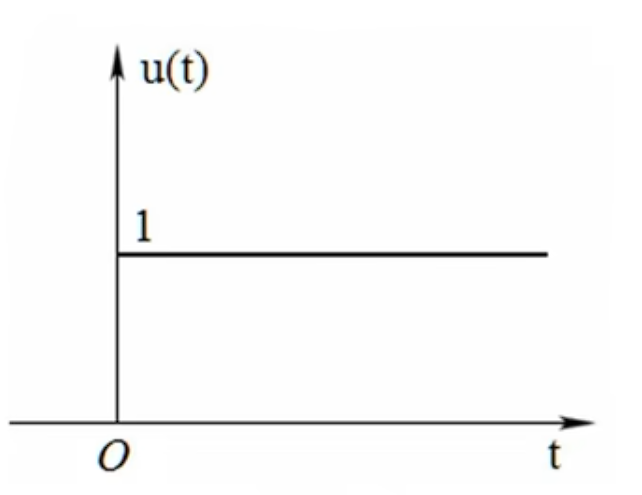
\includegraphics[width=0.4\textwidth]{Figure/阶跃函数.png}
                        \caption{单位阶跃函数}
                    \end{figure}
                        \item[2)] 时移阶跃：
                    \begin{equation*}
                        f(t)\rightarrow af(t-t_0)
                    \end{equation*}
                    \item[3)] 阶跃函数的性质
                        \begin{itemize}
                        \item[(1)] 简化某些函数的表示
                            \begin{itemize}
                                \item 上升：+
                                \item 幅度
                                \item 转折点
                                \item 例题：$f(t)=\epsilon (t+1)+\epsilon (t-1) -3\epsilon (t-2)+\epsilon(t-4)$
                            \end{itemize}
                        \item[(2)] 倒置：$f(t)\rightarrow -f(t)$
                        \item[(3)] 加权、数乘 $f(t)\rightarrow af(t)$
                        \item[(4)]  表示信号的作用区间（参考简化的例题得到一段为1的函数）$f(t)=[\epsilon (t-t_1)-\epsilon (t-t_2)]$起点-终点
                        \item[(5)] 积分：$\displaystyle \int_{-\infty}^{t} \epsilon (\tau)d\tau =t\epsilon (t)$
                        \item[(6)]  微分：$\displaystyle \frac{d\epsilon (t)}{dt}=\delta (t)$ 
                        \item[(7)]r(t)求微分 得到阶跃，阶跃求微分得到冲激函数  
                    \end{itemize}
                    \newpage
                    \item[2)] 冲激信号
                        \begin{itemize}
                            \begin{figure}[h]
                                \centering
                                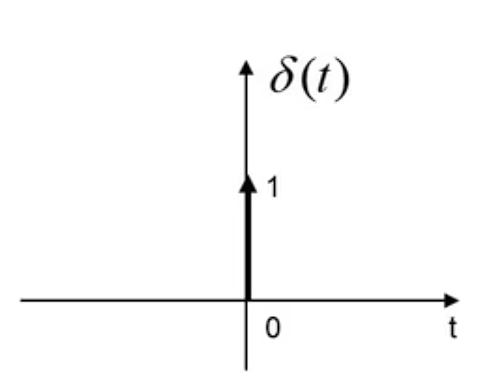
\includegraphics[width=0.4\textwidth]{Figure/冲激信号.png}
                                \caption{单位冲激信号}
                            \end{figure}
                            \item[(1)] $\displaystyle \int_{-\infty}^{\infty}\delta (t)dt=1$ 当且仅当t落在积分区间内才有意义，由此得出推导公式：
                            \begin{equation*}
                                \delta (t)=\int_{-\infty}^{\infty}\delta(t-t_0)dt=A
                            \end{equation*}
                            \item[(2)] 冲激偶函数$\delta'(t)$：奇函数（图后面补），冲激函数为偶函数
                            \item[(3)] 广义函数（奇异函数）：（手机上，后面补） 
                            \item[(4)] 冲激函数的特性
                                \begin{itemize}
                                        \item[1、] 加权特性：$f(t)\delta (t)=f(0)\delta (t)$，$f(0)$为有效点，拓展为$f(t)\delta (t-t_0)=f(t_0)\delta(t-t_0)$ 
                                    \item[2、] 筛选特性：$\displaystyle \int_{-\infty}^{\infty}f(t)\delta(t-t_0)dt=f(t_0)$
                    
                                    $\displaystyle \int_{-\infty}^{\infty}f(t)\delta(t)dt=f(0)\int_{-\infty}^{\infty}\delta(t)dt=f(0)$，积分区间外为0
                                    \item[3、] 尺度变换 $\displaystyle \delta(at)=\frac{1}{|a|}\delta(t)$ 
                                \end{itemize}
                                \newpage
                            \item[(5)] 单位冲激序列$\delta[n]$
                                \begin{equation}
                                    \delta[n]=
                                    \begin{cases}
                                        0 & n\neq 0\\
                                        1 & n=0
                                    \end{cases}                             
                                \end{equation}
                                \begin{figure}[h]
                                    \centering
                                    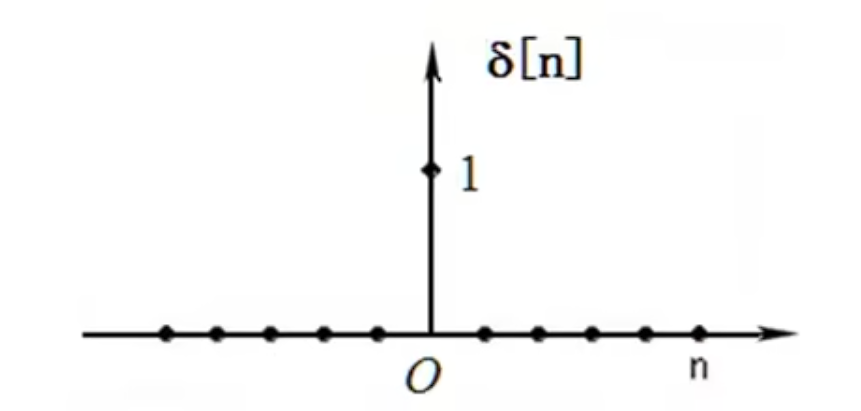
\includegraphics[width=0.4\textwidth]{Figure/离散单位脉冲序列.png}
                                    \caption{离散单位脉冲序列}
                                \end{figure}

                            
                        \end{itemize}
                    
                \end{itemize}
    \section{典型的系统}
        \subsubsection{线性系统}
        $x(t)\longrightarrow \boxed{\text{系统}}\longrightarrow y(t)$

        
            \begin{itemize}
                \item[1)] 若任意的$x(t)$经过某个系统得到$y(t)$ ，$x(t)\xrightarrow{\text{系统}}y(t)$，则有

                $ax(t)\xrightarrow{\text{系统}}ay(t)$（齐次性）
                \item[2)] 假设：
                
                任意$x_1(t)\xrightarrow{\text{系统}}y_1(t)$

                任意$x_2(t)\xrightarrow{\text{系统}}y_2(t)$则有：

                $x_1(t)+x_2(t)\xrightarrow{\text{系统}}y_1(t)+y_2(t)$（叠加性）
                \item[3)] 若一个系统\textbf{同时满足(1)、(2)}则称他为线性系统，否则为非线性系统
                \item[4)] 离散系统只需要把$x(t)$改成$x[n]$ 
                \item[5)] 线性系统的判据
                    \begin{itemize}
                        \item[(1)] 每一项都有$x$
                        \item[(2)] 每一项的$x$都是一次
                        \item[(3)] 此判据只有70\% 左右的正确率
                        \item[(4)] 例题：$y(t)=3x(t)+2x(t-2)$是否为线性。线性  
                        
                        而$\displaystyle y[n]=e^{x[n]}$是否为线性，此式子泰勒展开为$\displaystyle y[n]=1+x[n]+\frac{x^2[n]}{2!}+....+$因此为非线性
                    \end{itemize}
            \end{itemize}
        \subsection{时不变系统}
            \begin{itemize}
                \item[1)] 定义：$\forall x(t)\rightarrow y(t)$则$x(t-t_0)\rightarrow y(t-t_0),t_0\in R$ 
                \item[2)] 经验判据
                    \begin{itemize}
                        \item[(1)] $t$只在$x$的括号内
                        \item[(2)] $t$只能是$t$，不能是$-2t,2t,t^t$等其他函数
                    \end{itemize} 
            \end{itemize}
        \subsection{因果系统}
            \begin{itemize}
                \item[1)] 定义：如果一个系统任何时刻输出只决定于现在和过去的输入，就称该系统为因果系统。
                \item[2)] 经验判据：$x$括号内的数恒小于等于$y$括号内的数（要正负半轴下都小于）
            \end{itemize}
        \subsection{稳定系统}
            \begin{enumerate}
                \item 定义：$x(t)\rightarrow y(t)$，若$x(t)$有界，则$y(t)$有界，若$y(t)$无界则为非稳定系统
                \item 例：$y(t)=e^{x(t)}$是否为稳定的。
                
                        当$x(t)$输入有界时$y(t)$也有界

                        反例：微分器中的输入为阶跃，输出为冲激（无界）
            \end{enumerate}
        \subsection{无记忆系统}
            \begin{itemize}
                
            
            \item[1)] 定义：一个系统无记忆是指$y(t)$的值，仅只依赖于$x(t)$

            $y(t)=x(t-1)$，$y(t)$的值依赖于$(t-1)$所以这是记忆的

            \item[2)] 经验判据：$x$与$y$括号内的数完全一样
            \item[3)] 无记忆系统一定是因果系统
            \end{itemize}
        \subsection{可逆系统}
            \begin{itemize}
                \item[1)] 定义：$x(t)$能唯一写成$y(t)$的形式
                \item[2)] 例：$y(t)=x(t)^2,x(t)=\pm \sqrt{y(t)}$此时一个$x(t)$有两个$y(t)$与之对应为不可逆系统  
            \end{itemize}
\section{LTI系统的时域分析}
    \subsection{离散LTI系统卷积}
        \subsubsection{离散LTI系统卷积的原理}
        \begin{figure}[h]
                \centering
                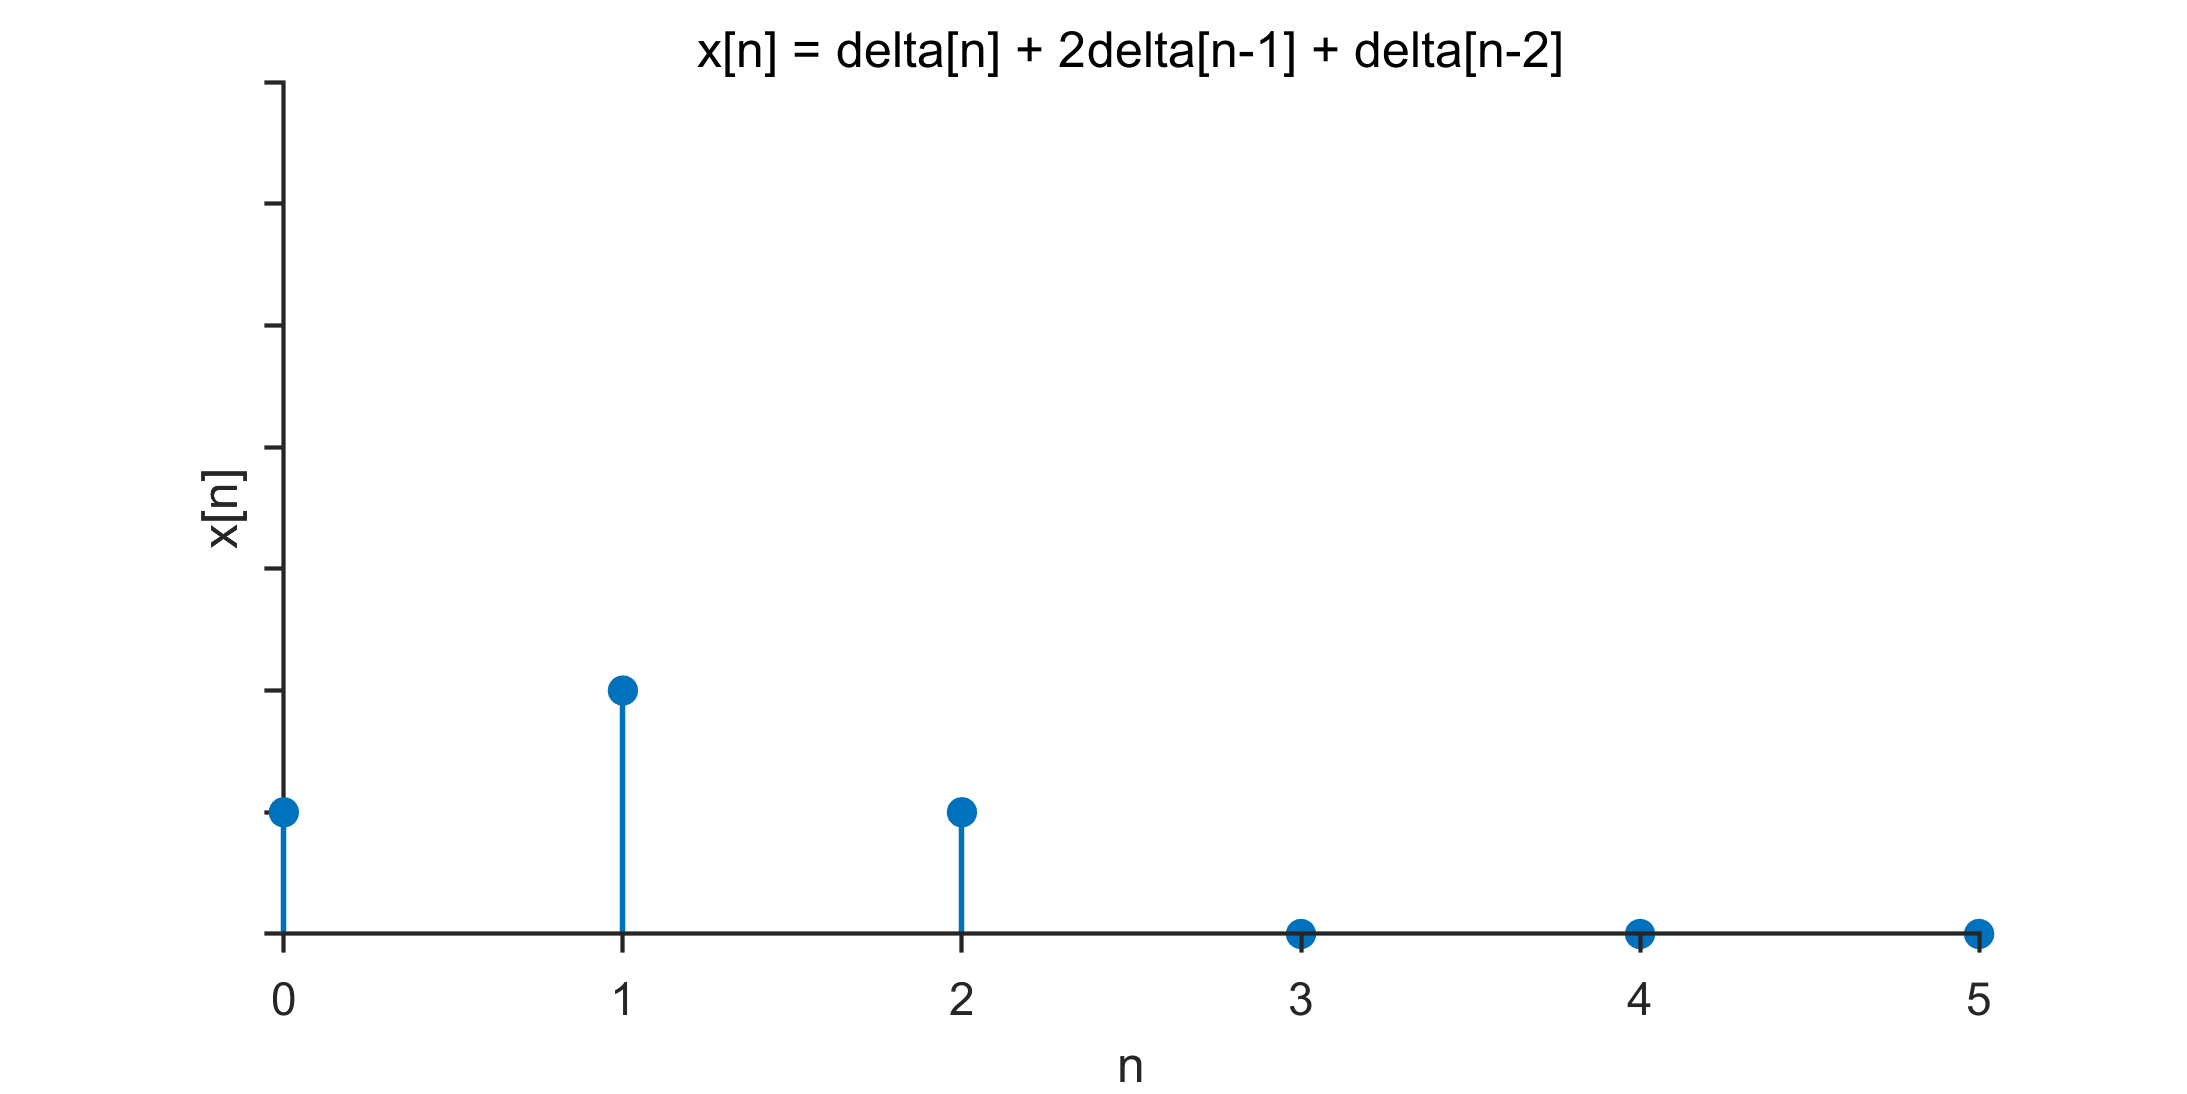
\includegraphics[width=0.7\textwidth]{Figure/第二章LTI离散卷积图像/图1_输入序列x[n].png}
                \caption{$x[n]$输入}
        \end{figure}
        一个离散$x[n]$可将其分解为如下$\delta[n]$的单位冲激
        \begin{figure}[h]
            \begin{minipage}{0.32\textwidth}
                \centering
                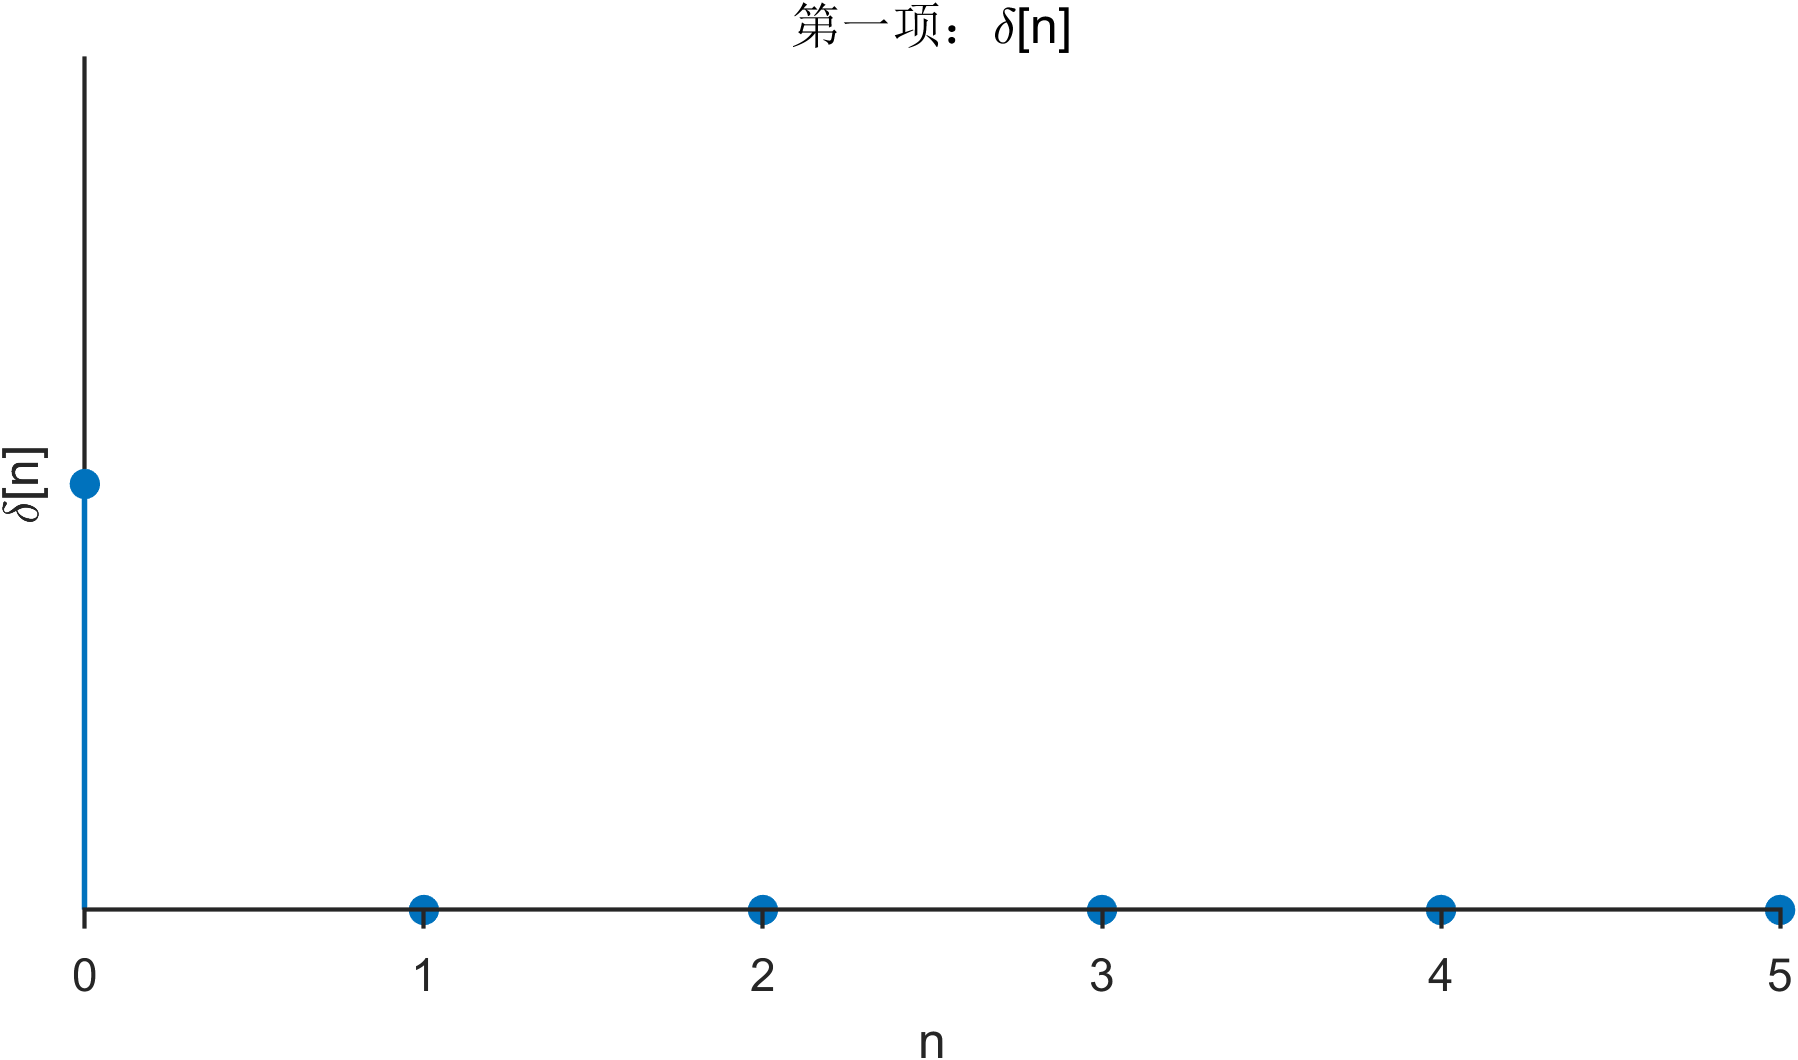
\includegraphics[width=1\textwidth]{Figure/第二章LTI离散卷积图像/图2_第一项δ[n].png}
                \caption{第一项$\delta[n]$}
            \end{minipage}
            \begin{minipage}{0.32\textwidth}
                \centering
                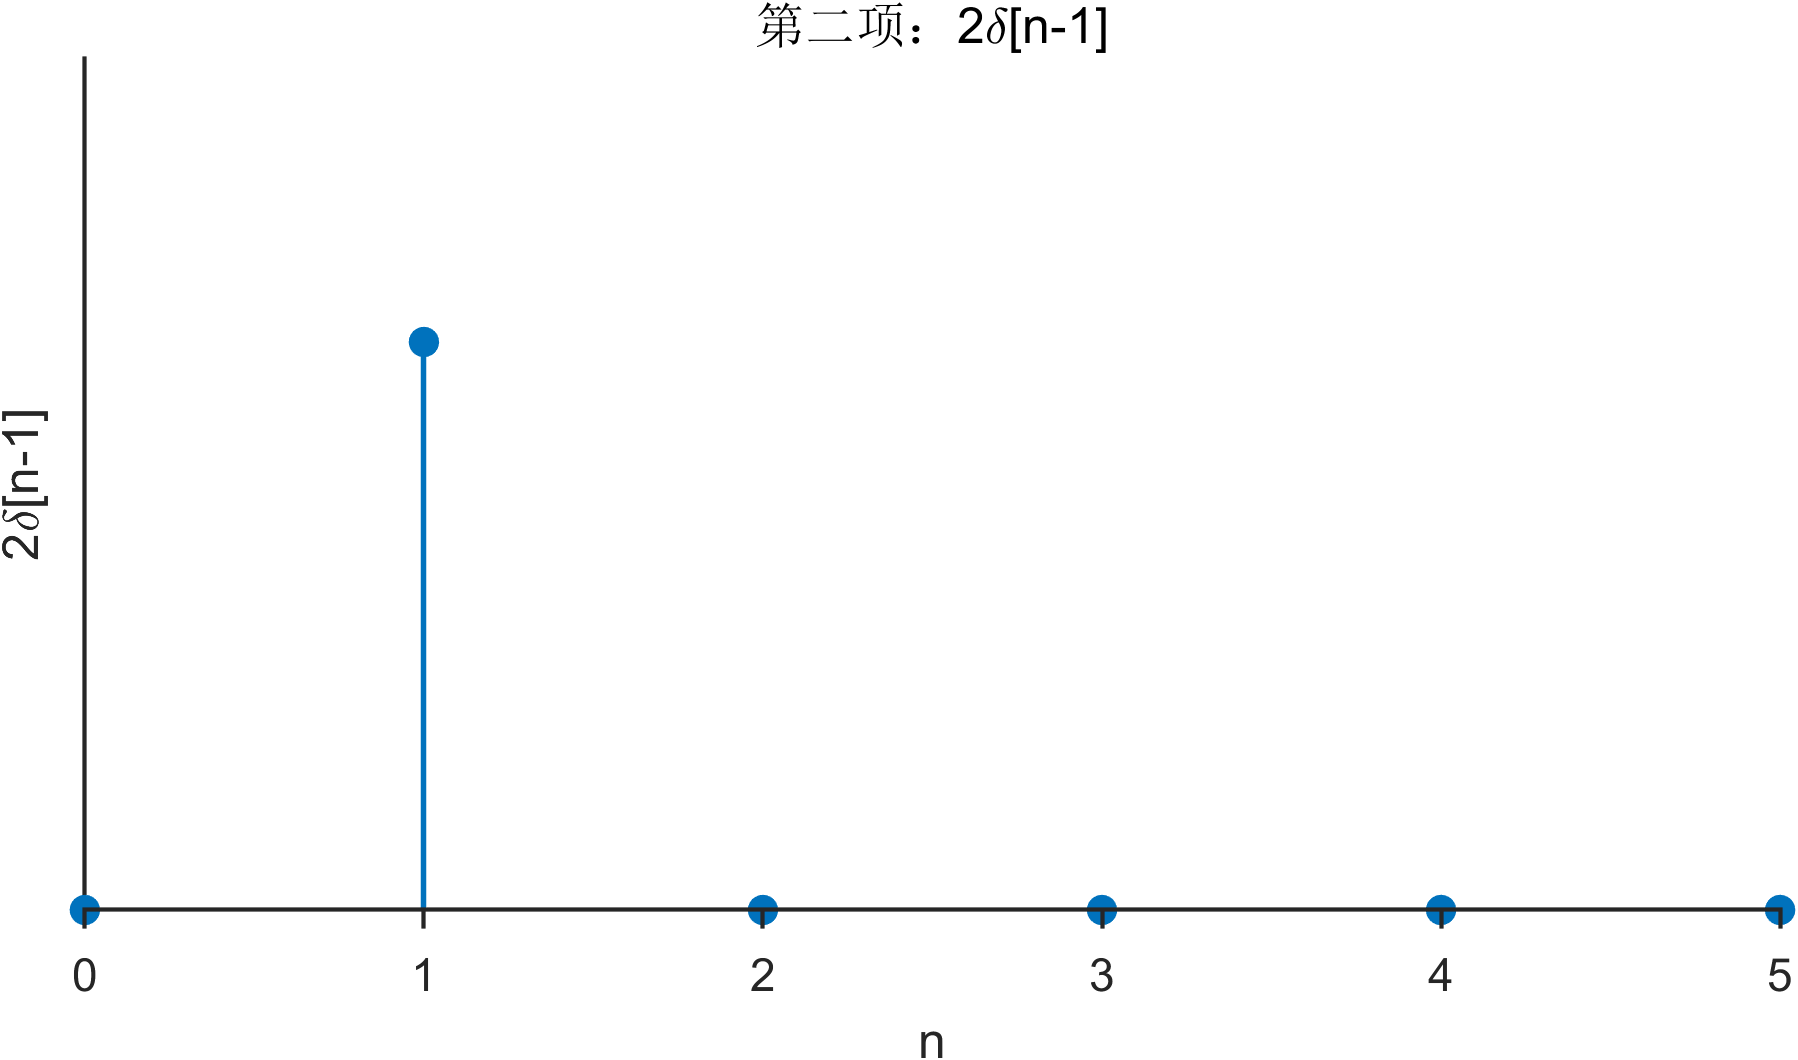
\includegraphics[width=1\textwidth]{Figure/第二章LTI离散卷积图像/图3_第二项2δ[n-1].png}
                \caption{第二项$\delta[n]$}
            \end{minipage}
            \begin{minipage}{0.32\textwidth}
                \centering
                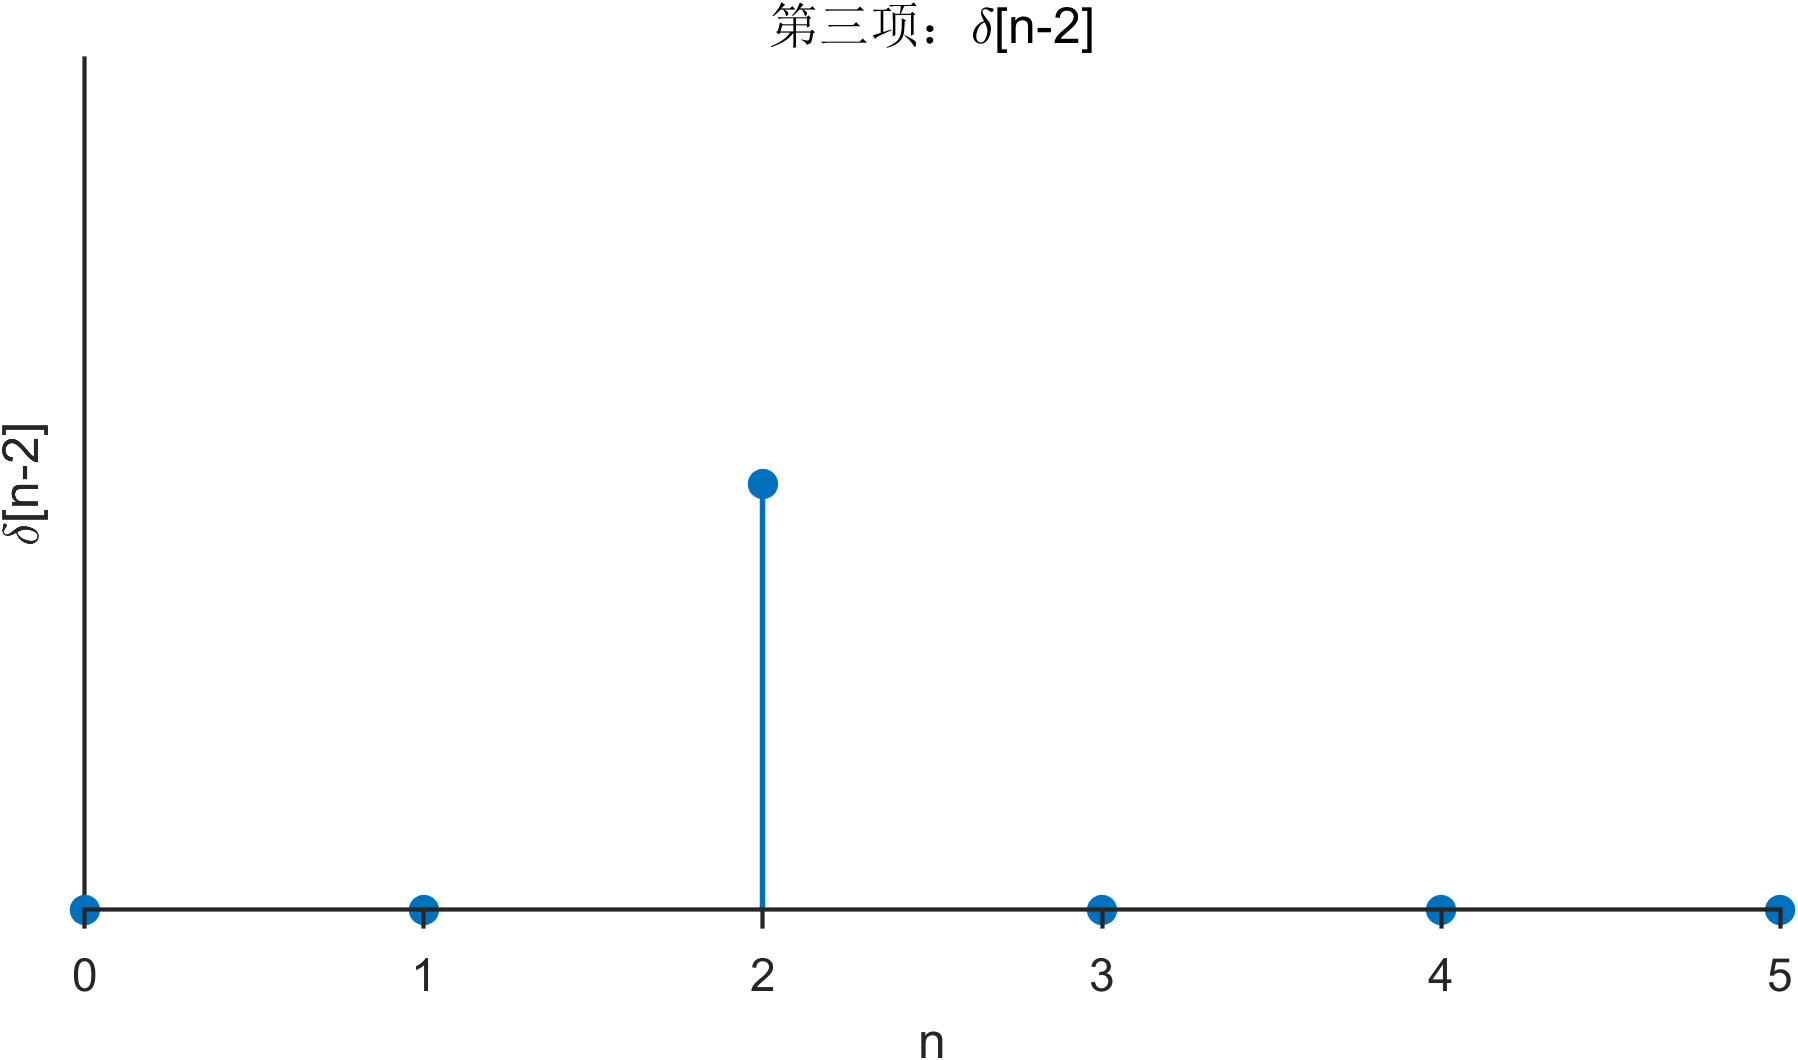
\includegraphics[width=1\textwidth]{Figure/第二章LTI离散卷积图像/图4_第三项δ[n-2].png}
                \caption{第三项$\delta[n]$}
            \end{minipage}
        \end{figure}

而这些个$\delta[n]$经过这个$LTI$系统会分别得到一个单位冲激响应（由齐次性得到）
        \begin{figure}[H]
            \begin{minipage}{0.32\textwidth}
                \centering
                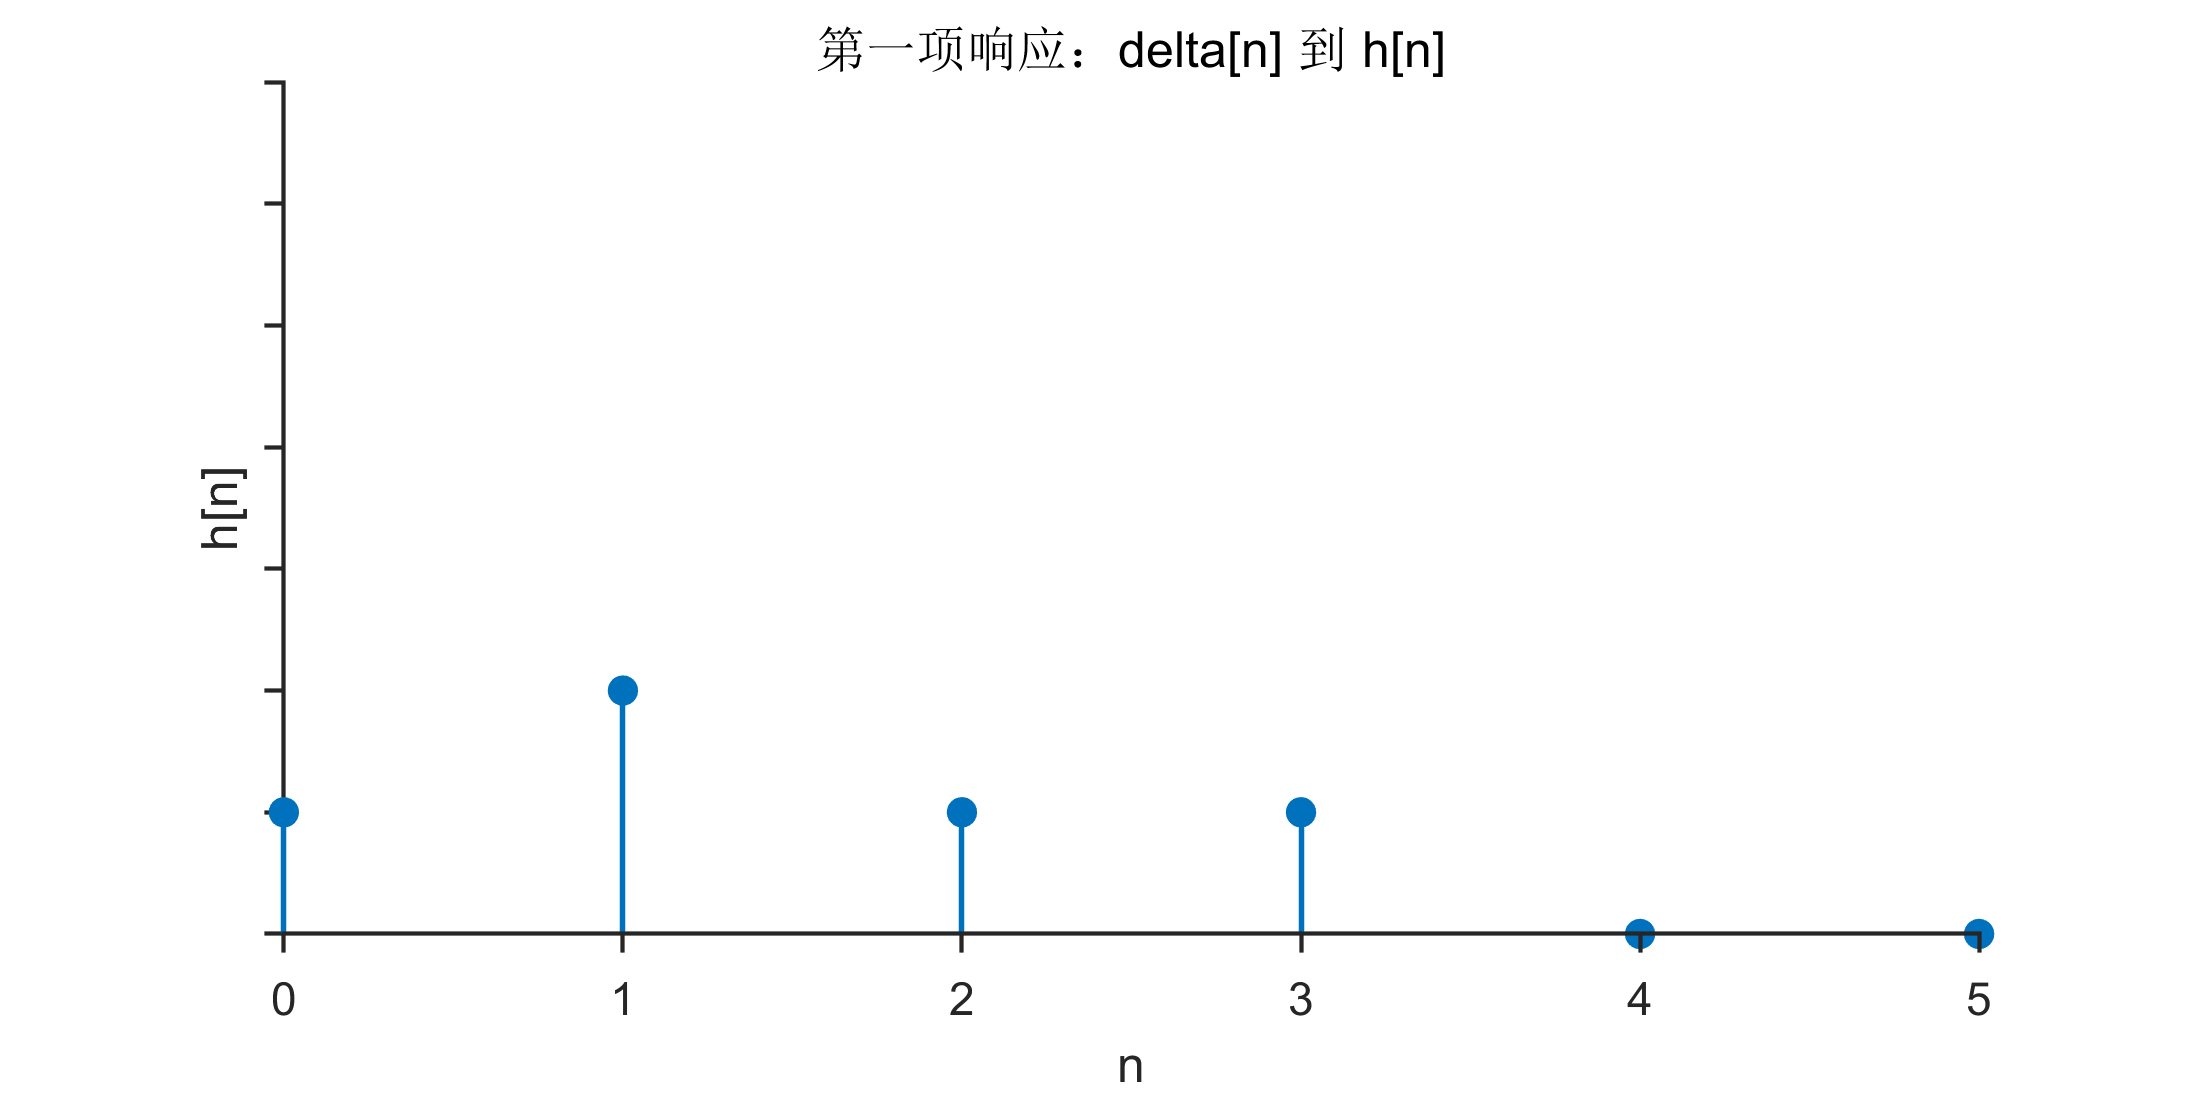
\includegraphics[width=1\textwidth]{Figure/第二章LTI离散卷积图像/图5_第一项响应h[n].png}
                \caption{第一项冲激响应$h[n]$}
            \end{minipage}
            \begin{minipage}{0.32\textwidth}
                \centering
                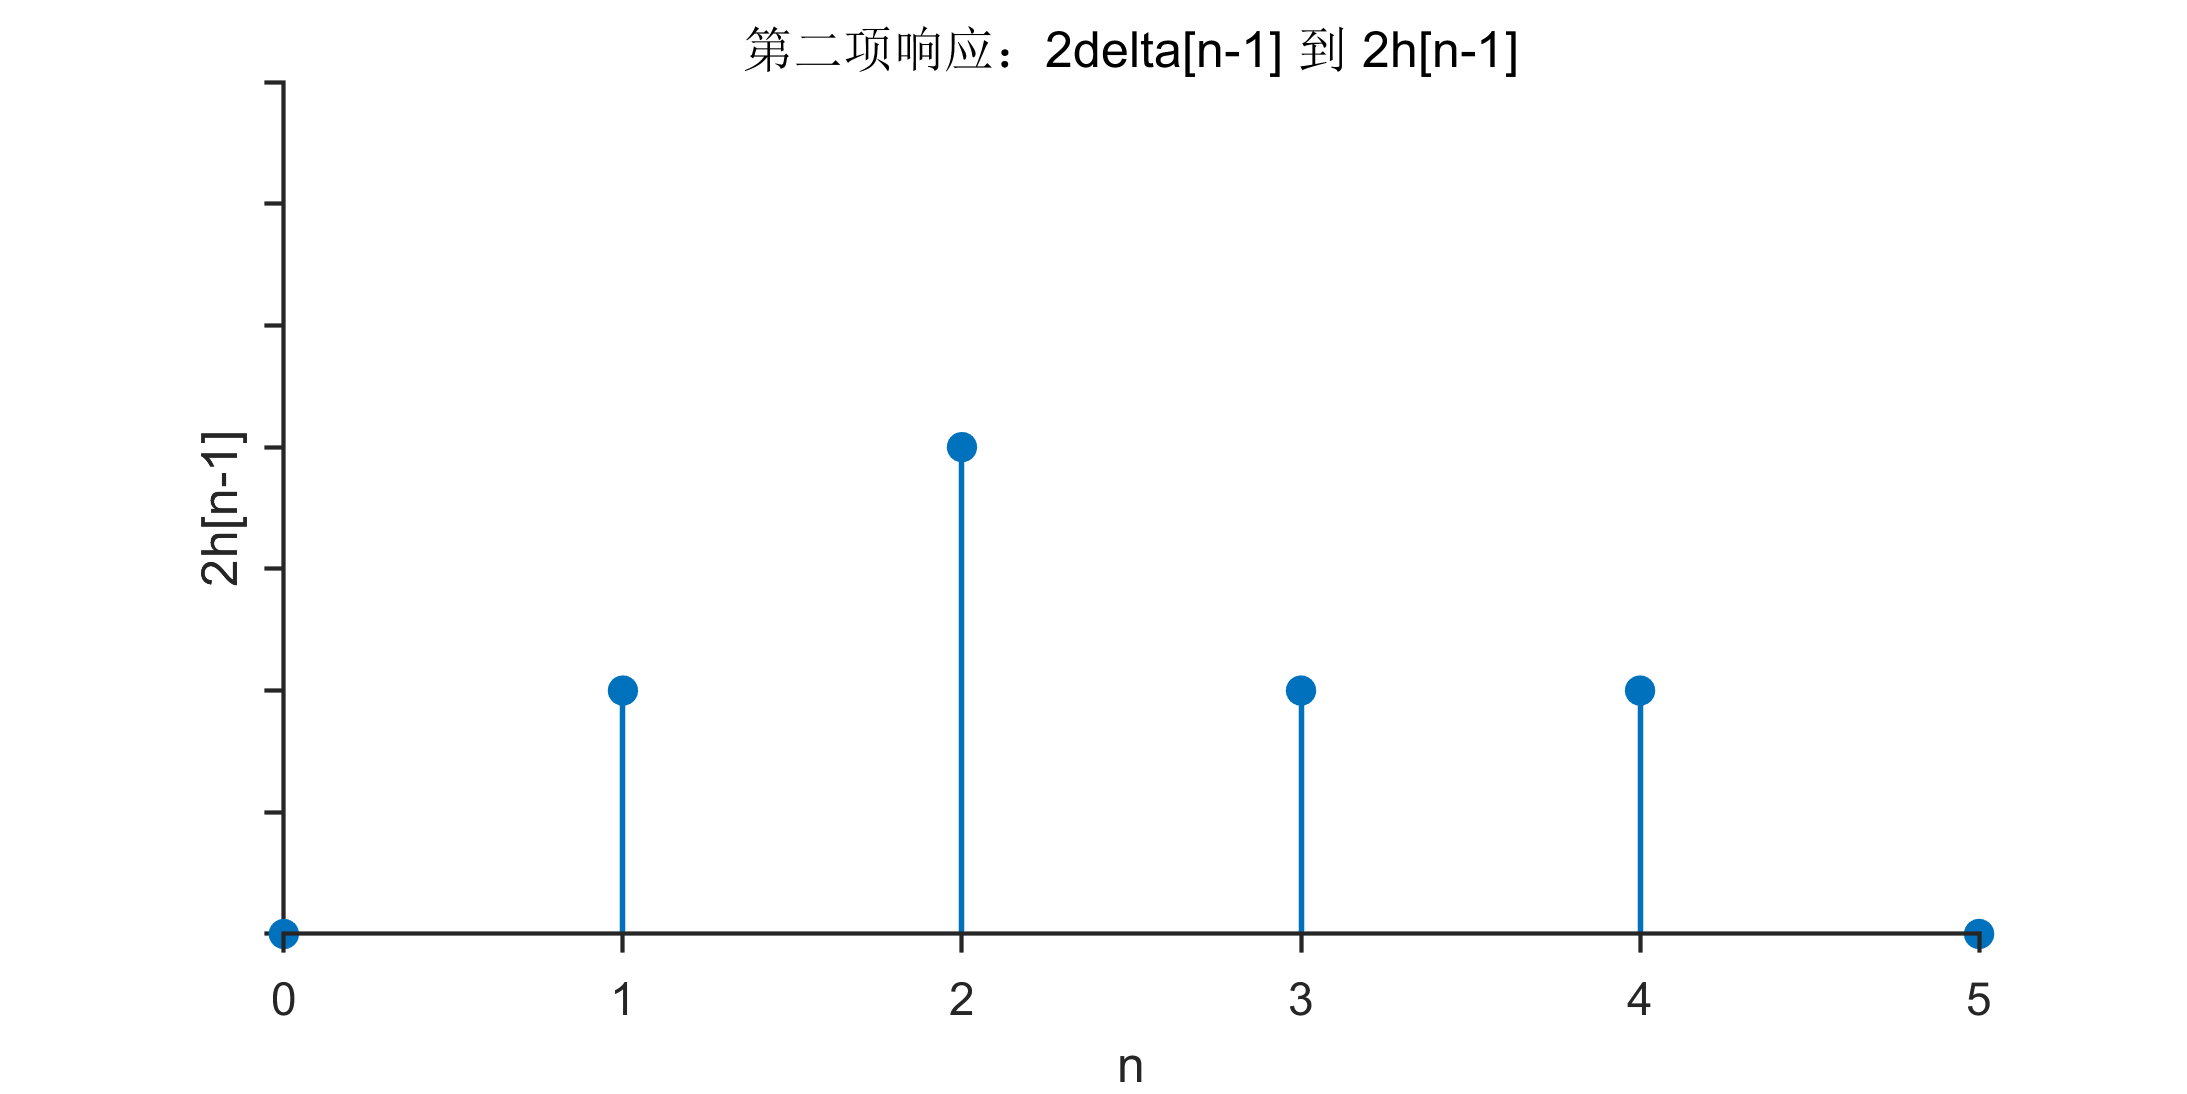
\includegraphics[width=1\textwidth]{Figure/第二章LTI离散卷积图像/图6_第二项响应2h[n-1].png}
                \caption{第二项冲激响应$h[n]$}
            \end{minipage}
            \begin{minipage}{0.32\textwidth}
                \centering
                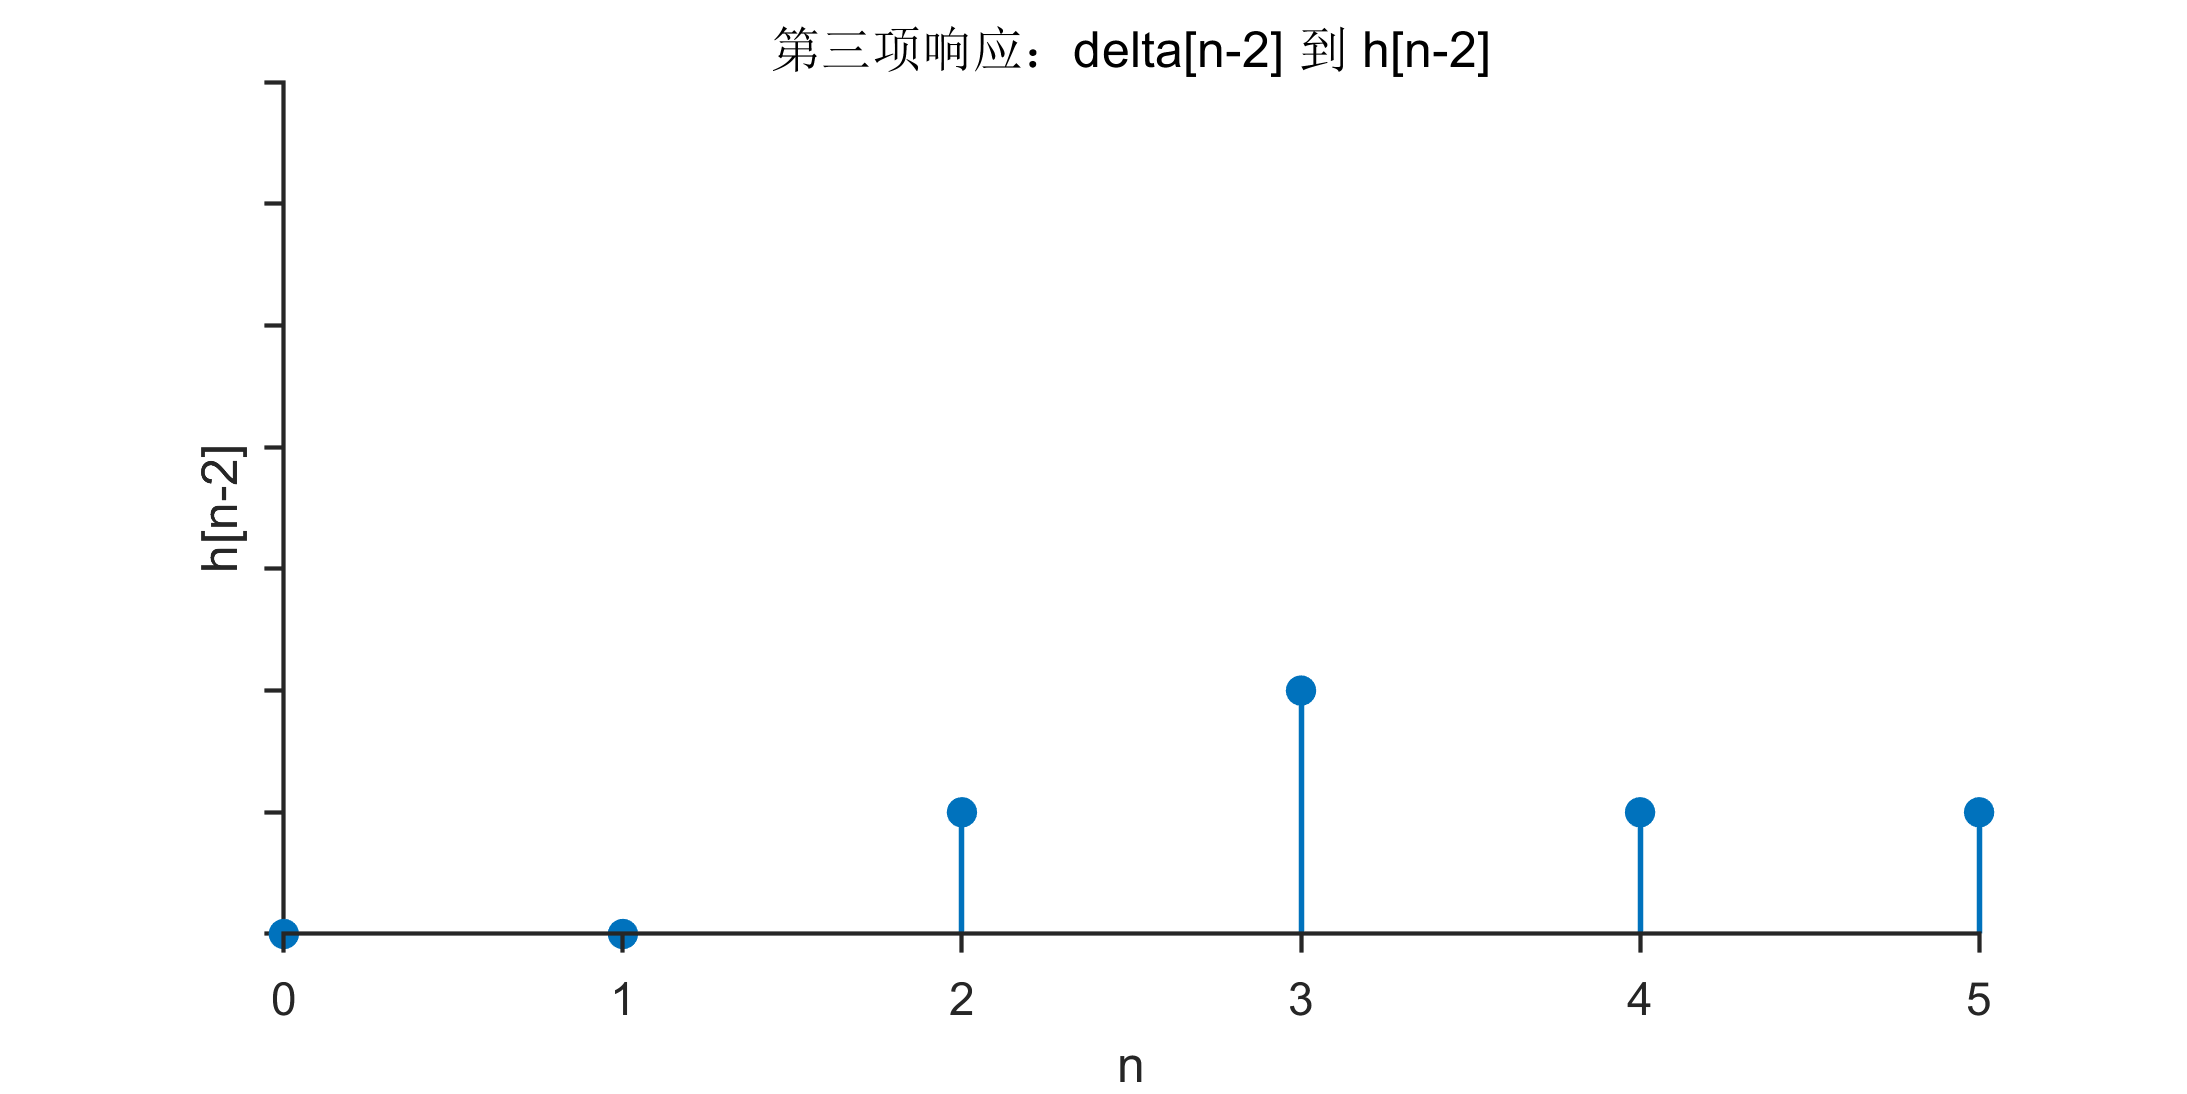
\includegraphics[width=1\textwidth]{Figure/第二章LTI离散卷积图像/图7_第三项响应h[n-2].png}
                \caption{第三项冲激响应$h[n]$}
            \end{minipage}
        \end{figure}


        此时再将每一个$\delta[n]$经过LTI系统得到的冲激响应相加就能得到最后卷积和的图像（由叠加性得到）
        \begin{figure}[h]
            \centering
            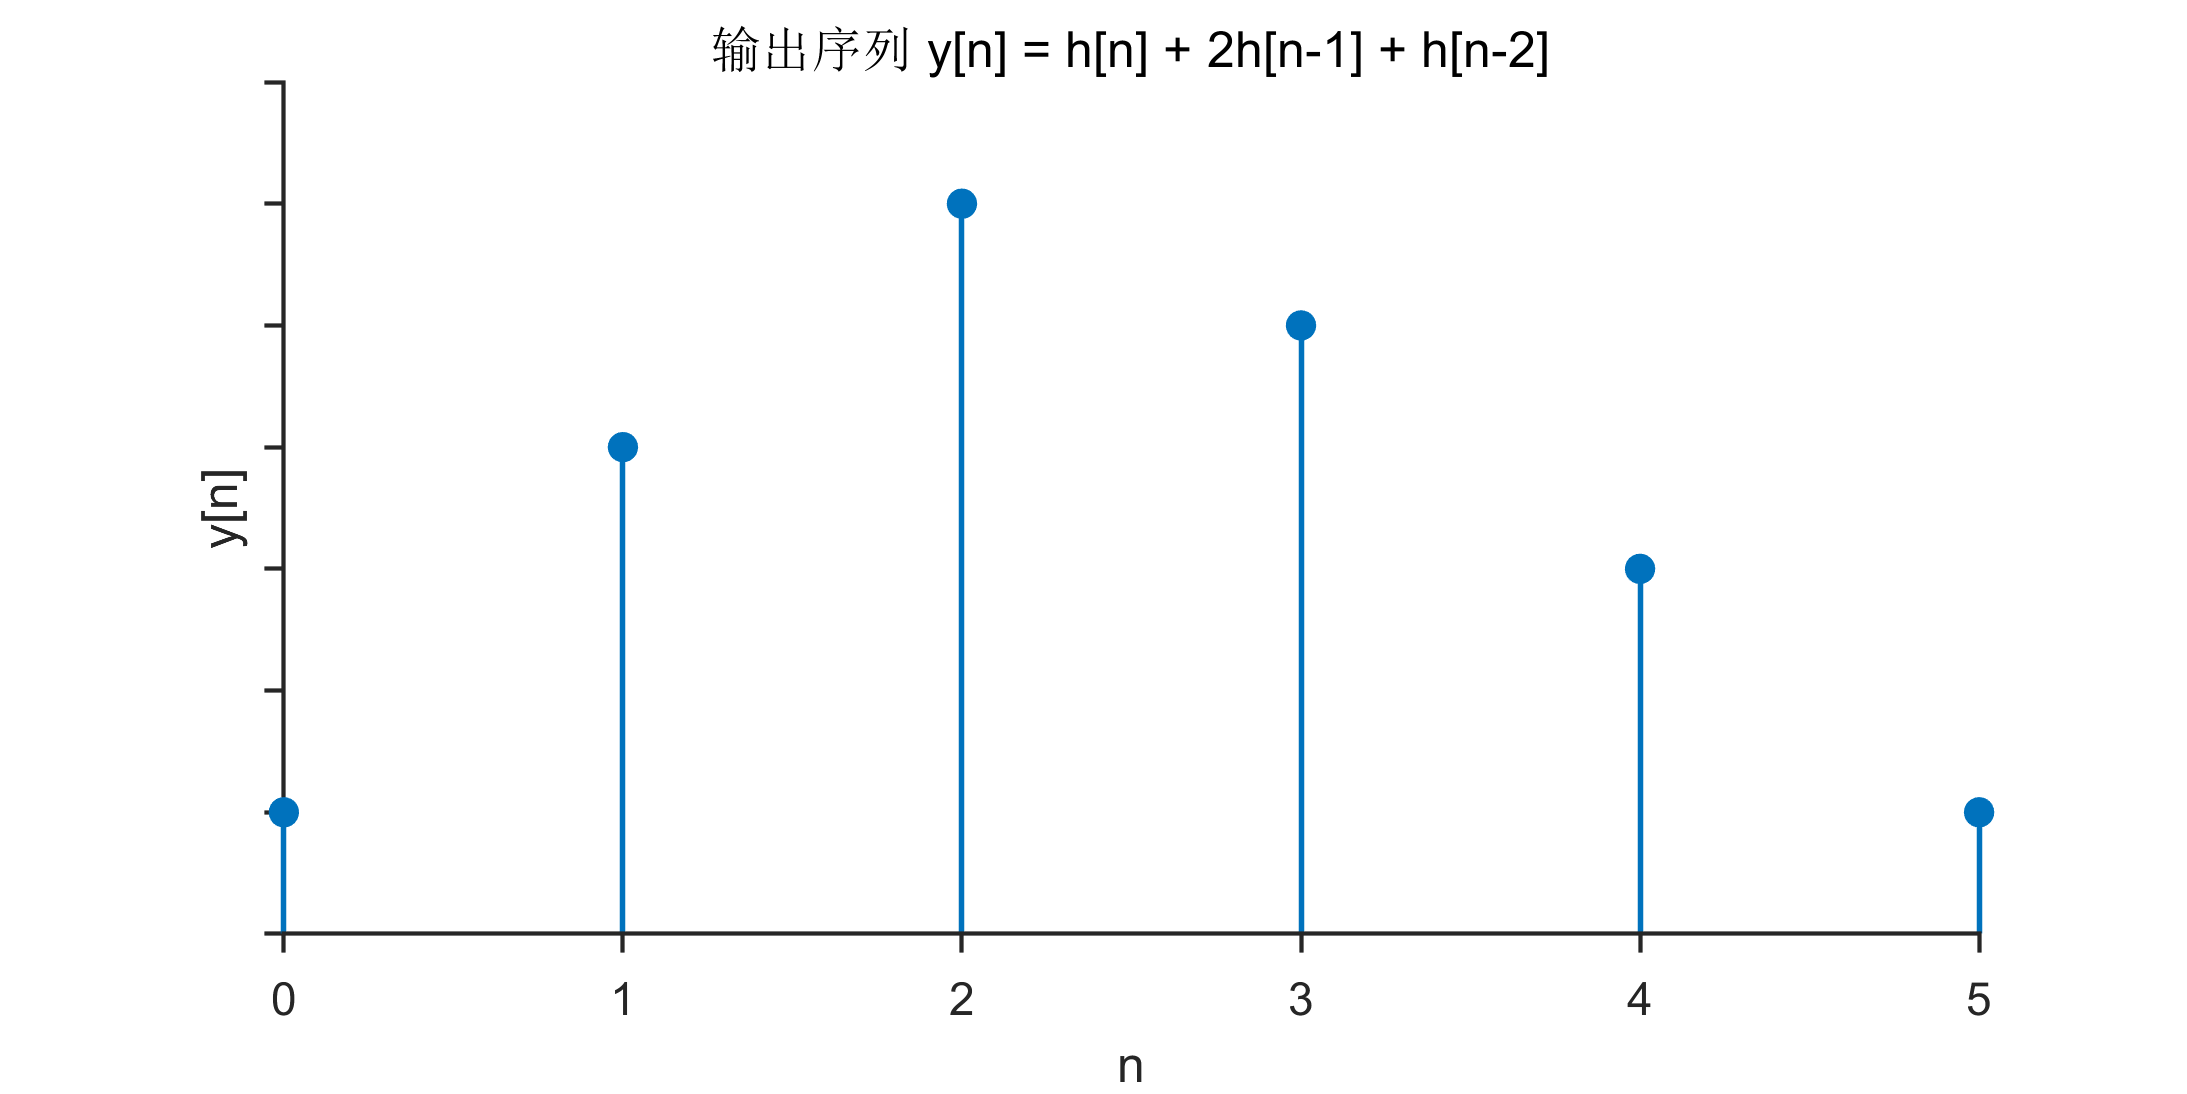
\includegraphics[width=0.7\textwidth]{Figure/第二章LTI离散卷积图像/图8_输出序列y[n].png}
            \caption{输出序列$y[n]$}
        \end{figure}

        因此，离散系统的卷积就是把$x[n]$分解为$\delta[n]$之后分别经过$LTI$系统得到各自的单位冲激响应而后叠加得到新的图像
        \begin{tcolorbox}[colback=blue!5!white]
        列表法求离散卷积和
        \begin{enumerate}
            \item 确定$y[n]=x[n]\ast h[n]$的取值范围：$y[n]$最左边（最右边）=$x[n]$最左边（最右边）+$h[n]$最左边（最右边）
            \item 列表：横着为$h[n]$依次从左到右的值，竖着为$x[n]$依次从左到右的值，然后$x[n]$乘$h[n]$的值
            \item 按照取值范围从最左边到最右边依次填入$x[n]$乘$h[n]$完相加的值
        \end{enumerate}
        \end{tcolorbox}
        
        例如图12：
            \begin{figure}[H]
                \centering
                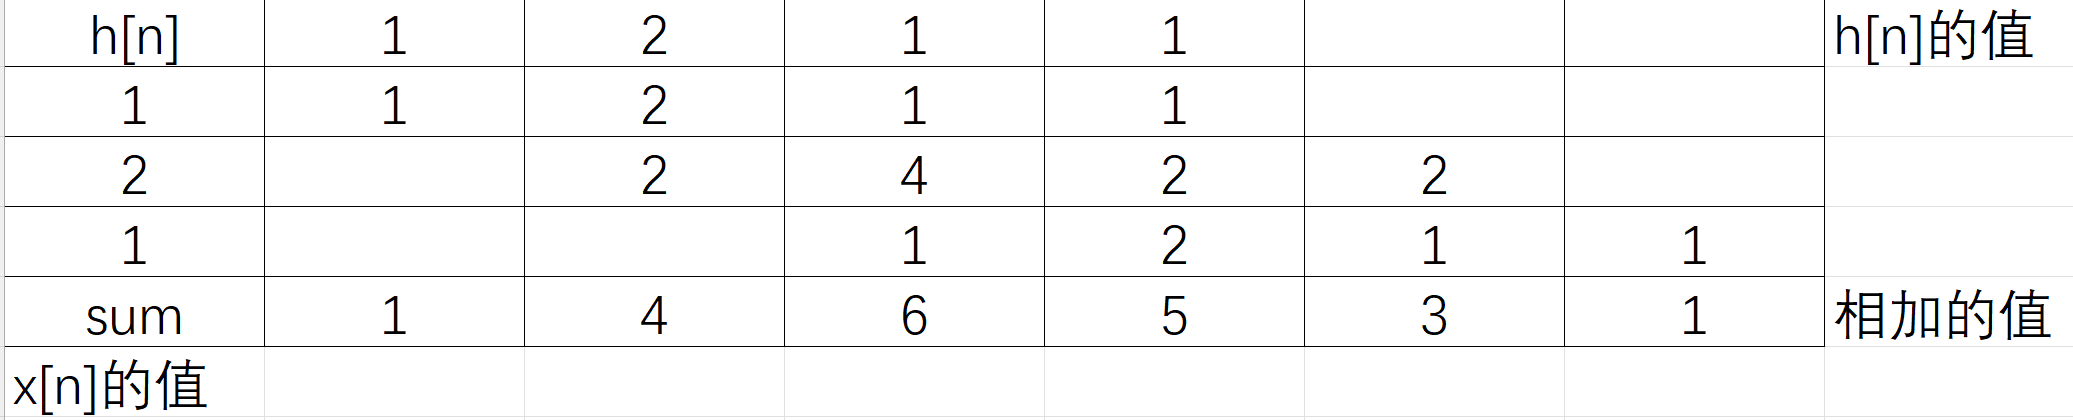
\includegraphics[width=0.8\textwidth]{Figure/第二章LTI离散卷积图像/列表法求离散卷积图像.png}
                \caption{列表法求离散卷积图像}
            \end{figure}

        注意$x[n]$与$x[n-1]$的值要错开，因为$LTI$系统具有时不变性，因此$x[n-1]$比$x[n]$要向右移一格
\end{document}